\section{Hashing-Based Remap Methodology}

Hash-based algorithms have gained attention as a promising alternative to traditional tree-based remap methods due to their simplicity and efficiency, especially in parallel computing environments. Earlier work by Robey et al. (2013) demonstrated that mesh operations such as remapping and neighbor-finding can be implemented using perfect hash functions, which ensure one unique value per bin and no collisions.

While perfect hashes are effective in structured mesh data, they can be inefficient in memory usage, especially when many bins remain unused. This leads to the concept of \textbf{compact hashing}, which improves memory efficiency by handling collisions while avoiding unnecessary allocations.

\subsection{Perfect Hash}

A perfect hash maps keys to values with no collisions, offering constant-time lookup. However, the hash table often needs to allocate memory for the entire domain, which is wasteful in sparse mesh data. The earlier implementations using perfect hashes showed performance improvements of 4--50$\times$ over CPU tree-based methods, and up to 20$\times$ faster on GPU.Earlier work by Robey et al. demonstrated hash-based remapping using perfect hashes for mesh operations~\cite{Robey2013}.


\subsection{Compact Hash}

To address the limitations of perfect hashing, Tumblin et al. introduced the compact hash, which is designed for sparse mesh data. In this scheme, the hash table uses sentinel values to indicate empty bins, and introduces some possibility of "misses" when a lookup retrieves a sentinel and must perform additional reads.

The compact hash is not injective; instead, it aims to avoid mapping many irrelevant keys by using a more selective hashing function. This reduces overall memory usage. Experimental studies, such as those by Alcantara et al., suggest that compact hash tables can achieve good performance when sized between $1.25N$ to $2N$ entries, where $N$ is the number of active mesh elements~\cite{Alcantara2009,Tumblin2010}.

\subsection{Advantages in Parallel Architectures}

The main advantage of hash-based methods over comparison-based (e.g., kD-tree) methods lies in their flat, predictable control flow. This makes them ideal for massively parallel environments like GPUs, where branching and cross-thread communication can severely hurt performance. With minimal synchronization requirements and efficient memory use, hash-based methods are well-suited for HPC platforms.

\begin{figure}[h]
  \centering
  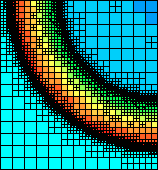
\includegraphics[width=0.75\textwidth]{./images/figure_p4_1.png}
  \caption{Overview of the hash-based remapping architecture. This figure illustrates the core logic and control flow of the multi-write, compact, and hierarchical hash methods.}
  \label{fig:hash_architecture}
\end{figure}
